\documentclass[a4paper]{report}

\usepackage[utf8]{inputenc}
\usepackage[T1]{fontenc}
\usepackage[french]{babel}
\usepackage{amsmath}
\usepackage{graphicx}
\usepackage{numprint}
\usepackage{enumitem}
\usepackage{scrextend}
\usepackage{a4wide}
\usepackage{float}
\usepackage{textcomp, gensymb}
\usepackage{booktabs}
\usepackage{array}
\usepackage{tabularx}
\usepackage{minted}
\usepackage{algpseudocode}
\usepackage{rotating}
\usepackage[toc,page]{appendix}
\usepackage[final]{pdfpages}
\usepackage[footnote]{acronym}
\usepackage[export]{adjustbox}
\usepackage[lofdepth,lotdepth]{subfig}
\usepackage{hyperref}
\usepackage[colorinlistoftodos]{todonotes}

\renewcommand{\labelenumii}{\theenumii}
\renewcommand{\theenumii}{\theenumi.\arabic{enumii}.}

\let\EndItemize\enditemize
\def\enditemize{\EndItemize\bigskip}

\newenvironment{absolutelynopagebreak}
  {\par\nobreak\vfil\penalty0\vfilneg
   \vtop\bgroup}
  {\par\xdef\tpd{\the\prevdepth}\egroup
   \prevdepth=\tpd}

\setlength{\parindent}{2em}
\setlength{\parskip}{1em}
\addtokomafont{labelinglabel}{\bf}

\begin{document}

%%%%%%%%%%%%%%%%%%
%%% First page %%%
%%%%%%%%%%%%%%%%%%

\begin{titlepage}
\begin{center}


\includegraphics[width=0.6\textwidth]{img/logo_polytech.png}\\[1cm]

{\large Informatique Industrielle en apprentissage}\\[0.5cm]

{\large Projet de Fin d'Étude}\\[0.5cm]

% Title
\rule{\linewidth}{0.5mm} \\[0.4cm]
{ \huge \bfseries Or-Box - Rapport final\\[0.4cm] }
\rule{\linewidth}{0.5mm} \\[1.5cm]

% Author and supervisor
\noindent
\begin{minipage}{0.4\textwidth}
  \begin{flushleft} \large
    \emph{Auteur :}\\
    M.~Pierre \textsc{Robillard}\\
  \end{flushleft}
\end{minipage}%
\begin{minipage}{0.4\textwidth}
  \begin{flushright} \large
    \emph{Encadrant :} \\
    M.~Frédéric \textsc{Rayar}\\
  \end{flushright}
\end{minipage}

\vfill

% Bottom of the page
{\large Version 0.1 du\\ \today}

\end{center}
\end{titlepage}

\tableofcontents
\listoffigures

\chapter{Introduction}
    \section{Domaine d'application}
    
    Le domaine d’application se limite à la OrBox --- un PFE pour le département d'Informatique Industrielle de Polytech Tours.
    Pour rappel, la Or-Box est un système destiné aux personnes souffrant de déficience visuelle.
    Elle a pour but de les aider au quotidien à reconnaître et distinguer des objets de la vie courante, et ce malgré leur handicap.
    
    \section{Porté du document}
    
    L’objet du document est de faire un retour d'expérience sur le déroulement du PFE dans son ensemble.
    Il se concentrera notablement sur la gestion de projet et les résultats obtenues.
    
    Pour mémoire, les spécifications du système sont décrites dans \cite{OBCdS}, la modélisation et l'analyse du système sont décrites dans \cite{OBMod}. La lecture préalable de ces derniers est recommandée.
    
\chapter{Retour d'expérience sur la gestion de projet}
\section{Planning prévisionnel \& réel}

La figure \ref{ganttinit} reprend le planning prévisionnel présenté dans le cahier de spécification, seulement elle n'en garde que les macros-tâches par souci de lisibilités.
La figure \ref{ganttfinal} montre à la même échelle l'avancement réel sur ces macros-tâches.
Les écarts notables sont :
\begin{description}
    \item[Tâche "électronique"] La fin réelle a été mi-décembre, au lieu de la planification début novembre.
    Ce retard est du a trois facteurs ; le premier concerne une légère sous-estimation du temps d'assemblage qui compte pour environ une semaine de délai, le deuxième concerne un problème technique lors de la phase de test (2 semaines) et le troisième concerne un problème de ressource pour la fabrication du PCB (3 semaines) --- plus de détail sur ces deux derniers points dans la section \ref{diff}.
    \item[Tâche "Image processing \& ML"] L'intégration de l'électronique dans le boitier étant une précédence à l'acquisition des images formant la base d'apprentissage, le travail sur le traitement d'image a été repoussé à mi-décembre.
    \item[Tâche "Serveur HTTP"] Cette tâche n'était pas prioritaire et ne faisait pas partie du chemin,  sa réalisation a été repoussée en vue de se concentrer sur la rédaction du cahier de spécification sur la période temps qui lui était initialement alloué.
\end{description}

\begin{figure}[H]
    \centering
    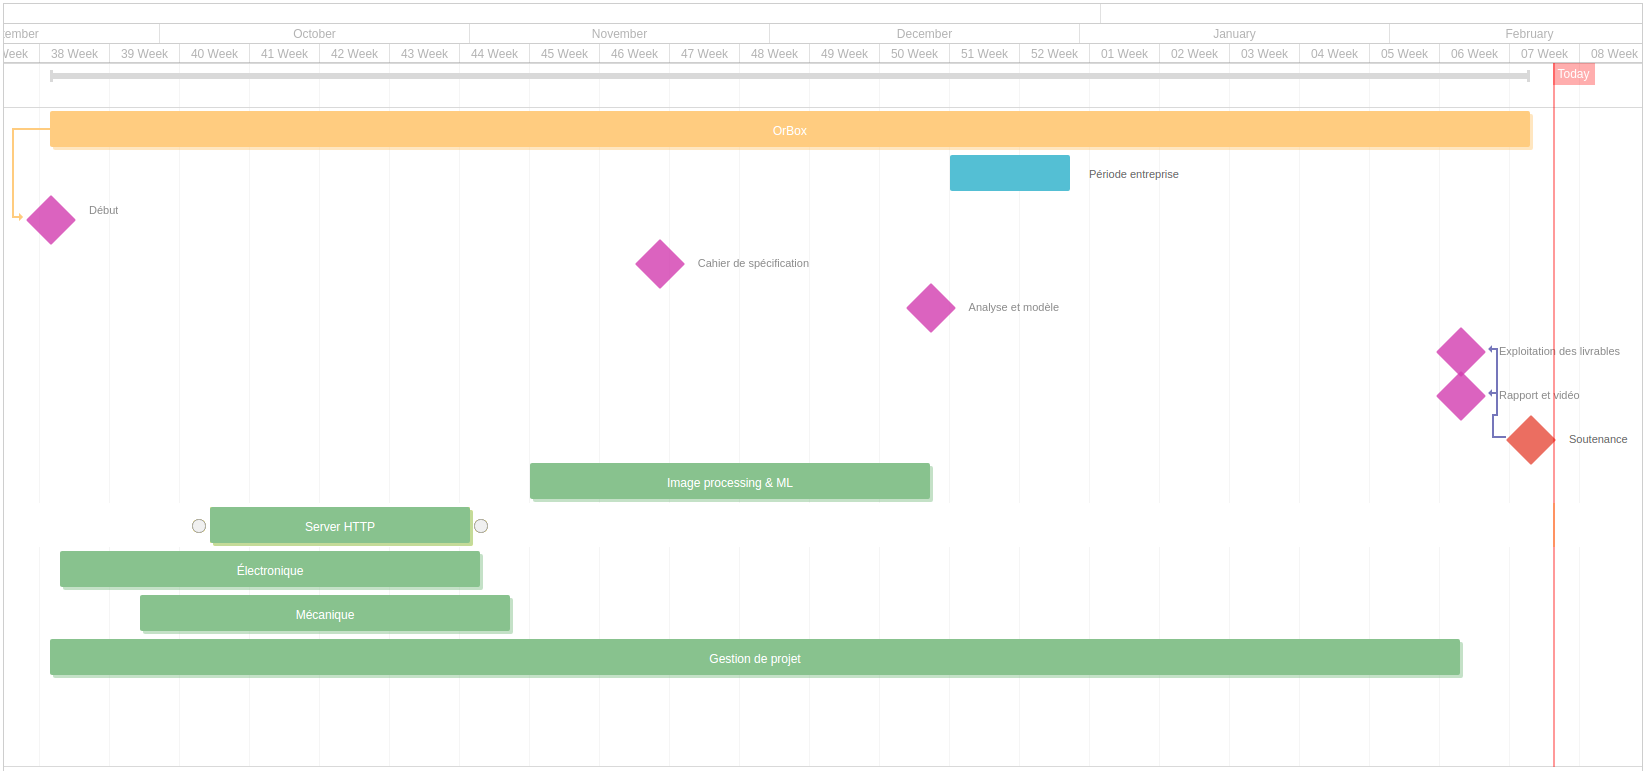
\includegraphics[width=\textwidth]{ganttproInit}
    \caption{Planning prévisionnel}
    \label{ganttinit}
\end{figure}

\begin{figure}[H]
    \centering
    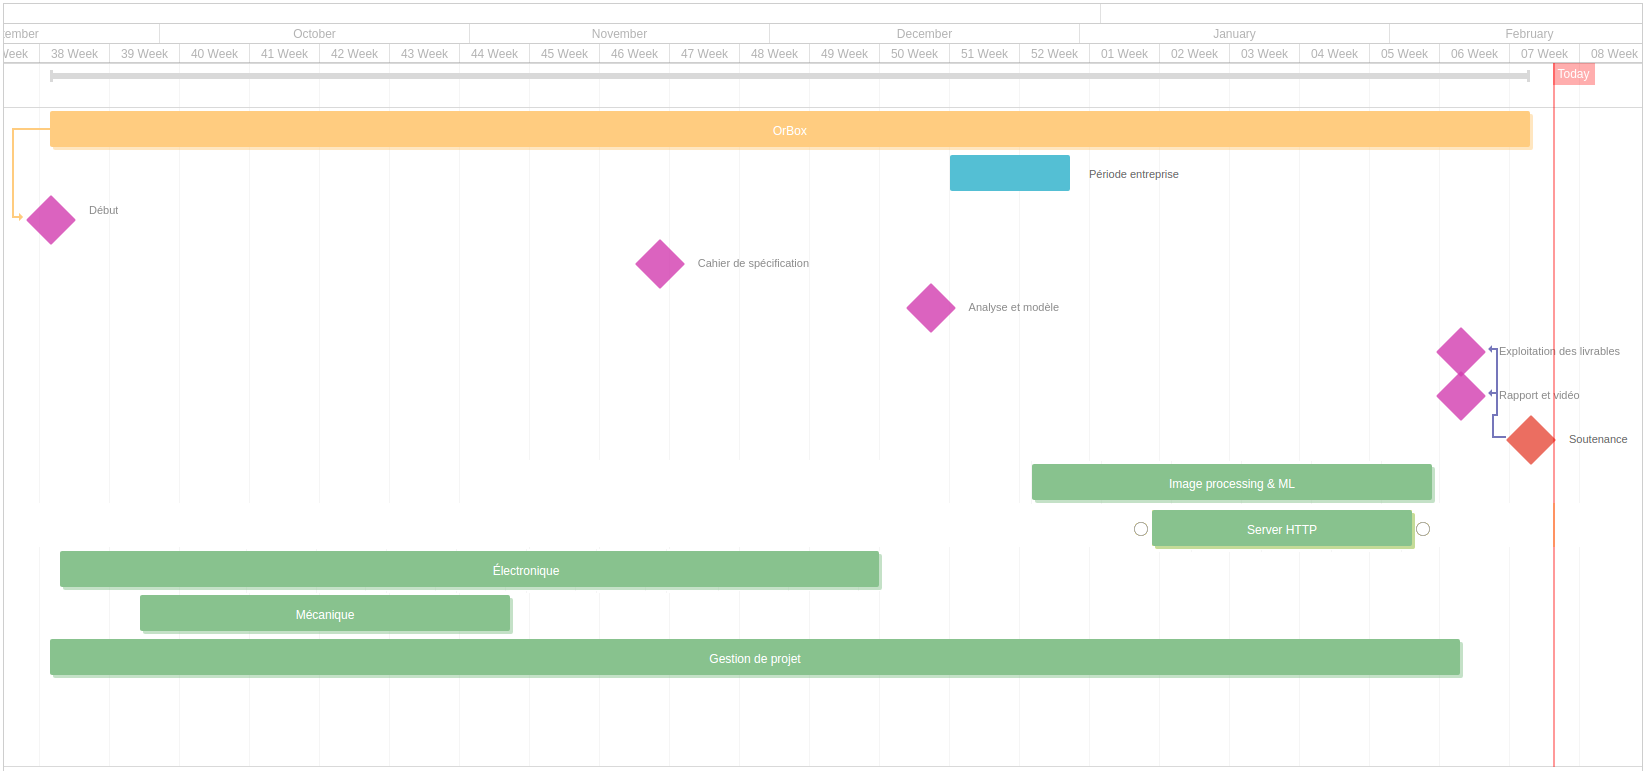
\includegraphics[width=\textwidth]{ganttproFinal}
    \caption{Planning réel}
    \label{ganttfinal}
\end{figure}

\section{Difficultés rencontrées}
\label{diff}


\chapter{Avancement du projet}
\section{Écart avec la spécification}
Voici la liste des différences entre la spécification et l'implémentation :
\begin{description}
    \item[L'interface d'administration.] Il s'agit de différences technologiques.
    D'abord envisagé comme étant une application écrite en Scala avec le framework Scalatra et une sérialisation des données sur MongoDB afin de monter en compétences sur ces nouvelles technologies, elle a finalement été écrite avec NodeJS et la sérialisation des données faites par écriture de fichiers JSON.
    Ce changement de technologies est dû à un manque de temps pour l'autoformation.
    \item[L'interface d'IHM embarqué] en charge du lancement d'un scénario de reconnaissance sur l'appuie du bouton physique de la Orbox n'a pas été écrite.
    Afin de tester toutefois ce scénario crucial, un bouton logiciel sur l'interface d'administration a été ajouté.
\end{description}

\section{Résultats des tests de performance}

\begin{table}[H]
\centering
\resizebox{\textwidth}{!}{%
\begin{tabular}{@{}llllllllllll@{}}
\toprule
\multicolumn{2}{l}{\textbf{Classe}} & \multicolumn{2}{l}{\textbf{Perimetère {[}px{]}}} & \multicolumn{2}{l}{\textbf{Circularité {[}\%{]}}} & \multicolumn{2}{l}{\textbf{Aire  {[}px^{2}{]}}} & \multicolumn{2}{l}{\textbf{\begin{tabular}[c]{@{}l@{}}Hauteur du rectangle\\ circonscrit {[}px{]}\end{tabular}}} & \multicolumn{2}{l}{\textbf{\begin{tabular}[c]{@{}l@{}}Largeur du rectangle\\ circonscrit {[}px{]}\end{tabular}}} \\
\textbf{Nom} & \textbf{Population} & \textbf{$\bar{x}$} & \textbf{$\sigma$} & \textbf{$\bar{x}$} & \textbf{$\sigma$} & \textbf{$\bar{x}$} & \textbf{$\sigma$} & \textbf{$\bar{x}$} & \textbf{$\sigma$} & \textbf{$\bar{x}$} & \textbf{$\sigma$} \\ \midrule
1 cent tail & 146 & 459.773 & \textit{24.206} & 0.891 & \textit{0.043} & 14,986.616 & \textit{1,315.304} & 126.607 & \textit{6.984} & 141.106 & \textit{9.116} \\
2 cents tail & 185 & 538.197 & \textit{28.429} & 0.892 & \textit{0.036} & 20,577.589 & \textit{1,955.259} & 151.506 & \textit{9.225} & 163.784 & \textit{10.186} \\
5 cents tail & 100 & 600.623 & \textit{24.398} & 0.886 & \textit{0.05} & 25,470.67 & \textit{2,399.964} & 169.136 & \textit{8.064} & 183.457 & \textit{9.643} \\
10 cents tail & 91 & 554.009 & \textit{17.996} & 0.892 & \textit{0.041} & 21,845.357 & \textit{1,931.995} & 156.86 & \textit{9.101} & 168.87 & \textit{8.329} \\
20 cents tail & 131 & 630.765 & \textit{20.307} & 0.884 & \textit{0.05} & 27,977.782 & \textit{2,009.784} & 177.785 & \textit{8.471} & 191.908 & \textit{8.294} \\
50 cents tail & 95 & 686.518 & \textit{24.688} & 0.881 & \textit{0.064} & 32,990.795 & \textit{2,636.762} & 194.756 & \textit{8.917} & 207.497 & \textit{11.377} \\
1 euro tail & 107 & 665.33 & \textit{29.773} & 0.874 & \textit{0.082} & 30,641.626 & \textit{2,144.526} & 187.928 & \textit{5.305} & 200.429 & \textit{8.841} \\
2 euros tail & 66 & 717.925 & \textit{8.798} & 0.903 & \textit{0.012} & 37,058.674 & \textit{1,017.615} & 206.697 & \textit{5.75} & 218.561 & \textit{4.034} \\ \bottomrule
\end{tabular}%
}
\caption{Moyenne et écart par classe pour les descripteurs basé sur les contours}
\label{stats}
\end{table}

Avec le retard pris pour la fabrication du circuit imprimé, il m'a resté moins de temps qu'escompté pour testé toutes les architectures architectures de classificateurs imaginés.
Heureusement la qualité des descripteurs choisis a permis d'atteindre des résultats satisfaisants rapidement.

Afin de mesurer la qualité des descripteurs la moyenne et l'écart type de chaque a été calculés.
Le résultat des ces mesures est visible dans la table \ref{stats}, le même travail a été effectué sur les histogrammes de teintes.
Ces calculs et leurs représentations graphiques ont été intégrés à l'interface d'administration du système afin d'aider l'utilisateur à paramétrer correctement sa Orbox.
On arrive ainsi à confirmer notre prédiction que le descripteur \emph{circularité} ne discrime pas suffisament les différentes classes entre elles dans le cas des pièces de monnaie.

\begin{table}[H]
\centering
\resizebox{\textwidth}{!}{%
\begin{tabular}{@{}lll@{}}
\toprule
\textbf{Descripteurs utilisés} & \textbf{Classificateur} & \textbf{Erreur moyenne} \\ \midrule
Aire et 60 barres d'histogramme & 1-NN 150-fold & 20.17\% \\ \midrule
Aire et 60 barres d'histogramme & 9-NN 150-fold & 22.14 \% \\ \hline
\begin{tabular}[c]{@{}l@{}}Aire, Perimètre, hauteur et largeur du rectangle\\ 15/42 barres d'histogramme\end{tabular} & SVM RBF 20-fold & 12.61\% \\ \midrule
\begin{tabular}[c]{@{}l@{}}Aire, Perimètre, hauteur et largeur du rectangle\\ 15/42 barres d'histogramme\end{tabular} & SVM Sigmoïd 20-fold & 78.23\% \\ \midrule
\begin{tabular}[c]{@{}l@{}}Aire, Perimètre, hauteur et largeur du rectangle\\ 15/42 barres d'histogramme\end{tabular} & SVM CHI2 20-fold & 7.42\% \\
\bottomrule
\end{tabular}%
}
\caption{Résultat obtenu pour 921 échantillons parmi 8 classes}
\label{SVM}
\end{table}

\chapter{Rapport financier}

Les coûts financiers de la Orbox ont été répartis sur les deux années.
Le tableau \ref{finance} donne l'estimation du prix du prototype.
Il est difficile d'estimer le coûts de production à partir de celui-ci.
En effet de nombreuses économies d'échelle seraient possibles ; aussi il souvent imposé une quantité minimum sur l'achat des composants électroniques.
L'annexe \ref{farnell} donne le détail de cette commande, on y voit que de nombreuses références n'apparaissant qu'une fois sur la BOM --- i.e. des résistances --- ont nécessité l'achat de 10 composants discrets.
Cependant tous n'ont pas été achetés en vain, car n'étant pas soudeur-câbleur de formation mon taux de soudure raté est élevé.

\begin{table}[H]
\centering
\begin{tabular}{@{}lll@{}}
\toprule
\textbf{Commandes} & \textbf{Fournisseurs} & \textbf{Coût} \\ \midrule
Composants électronique & Farnell & 128.75 € \\ 
Fabrication PCB & Euro-cricuit & 37.84 € \\ 
Camera USB & Amazon & 47.40 € \\ 
Raspberry Pi & RadioSpare & 34.95 € \\ 
Impression 3D & Polytech & - \\ 
Plexyglass, diffuseur   & & \textit{Don} \\ \midrule
\multicolumn{2}{r}{\textbf{Total}} & \textit{248.94 €} \\ \bottomrule
\end{tabular}
\caption{Récapitulatif des achats}
\label{finance}
\end{table}

\chapter{Conclusion}
Malgré une gestion du temps plus dure que prévu, le projet aboutit finalement sur une réussite des objectifs convenus avec la MOA en début de projets.
C'est à dire, qu'un prototype fonctionnel a été obtenu --- originalement, il avait été stipulé \emph{pleinement fonctionnel}, ces dernières finitions seront apportés dans le cadre des portes ouvertes --- l'objectif souhaité d'un taux de reconnaissance de 90\% minimum le cas d'utilisation des pièces de monnaie d'euros aété atteint.

\bibliographystyle{alpha}
\bibliography{mybib}
\begin{appendices}

\end{appendices}

\end{document}
